\section{Experiments}

We organize the evidence around three questions: whether learned directions
create selective intervention paths, which internal signals forecast those
paths, and whether those forecasts improve strength decisions. We report the
frozen confirmatory study here; the Supplementary Material adds protocol
details, uncertainty estimates, and analyses not shown in the main paper.

\subsection{Frozen Multidomain Study}

The benchmark contains 3,000 records from nine public sources: MMLU-Pro,
MMLU-Redux 2.0, AI2 ARC, OpenBookQA, SciQ, LiveBench reasoning and math,
HellaSwag, and QASC
\citep{wang2024mmlupro,gema2024mmluredux,clark2018arc,
mihaylov-etal-2018-suit,welbl-etal-2017-crowdsourcing,white2025livebench,
zellers-etal-2019-hellaswag,khot2020qasc}. The collection spans fourteen
academic, scientific, commonsense, mathematical, and reasoning domains. A
schema-constrained generation step converts each source item into disjoint
direction-fitting statements, three record-specific target probes, and three
semantic-neighbor probes; four globally balanced capability probes are assigned
per record. The worked example below traces one source item from fitting
evidence to evaluation probes and its resulting path label. Dataset composition,
validation, and additional examples appear in the Supplementary Material.

\begin{center}
\centering
\small
\setlength{\tabcolsep}{2.4pt}
\captionof*{table}{\textbf{Worked example.} One frozen record from construction to path label; direction-fitting statements and evaluation probes are disjoint.}
\begin{tabular}{@{}p{0.20\columnwidth}p{0.74\columnwidth}@{}}
\toprule
Object & Frozen example \\
\midrule
Source & MMLU-Redux 2.0 chemistry: Suppose that the 13C nuclei in a molecule in a 600 MHz spectrometer can be 100\% polarized (p = 1). If T1 = 5.0 s, how long does it take for p to reach a value equal to twice the thermal equilibrium polarization at 298 K? \\
Fit evidence & Positive statement: The polarization reaches twice the thermal equilibrium value in 72.0 seconds. Contrast statement: The polarization reaches twice the thermal equilibrium value in 56.6 seconds. \\
Target probe & Prompt: After full polarization, how long until it reaches twice thermal equilibrium?; candidate answers: 72.0 s vs. 56.6 s. \\
Neighbor probe & Prompt: The spin-lattice relaxation time T1 for 13C in this experiment is; candidate answers: 5.0 s vs. 10.0 s. \\
Capability probe & Prompt: An object in motion tends to stay in motion unless acted upon by an external force. This is; candidate answers: Newton's first law vs. Newton's second law. \\
Measured path & Mean difference, layer 11: suppression onset $-0.25$; positive neighbor onset $0.5$; no enhancement or capability onset. \\
Labels & Target=1, N-dmg.=1, C-dmg.=0, Clean suppression=1, Clean=1. \\
\bottomrule
\end{tabular}

\end{center}


We evaluate Qwen3-1.7B-Base \citep{yang2025qwen3} at two middle-depth
Transformer blocks, reported as blocks 7 and 11 by the model implementation and
selected using a 500-record layer-selection subset
(Figure~\ref{fig:layer-selection}). We
compare five direction constructions over a signed coefficient sweep. Random
directions calibrate target and collateral thresholds, while the weak response
at $|\alpha|=0.1$ is disjoint from the stronger coefficients used to define
confirmatory outcomes. Table~\ref{tab:main-results} defines the reported path
rates, and prediction folds hold out complete records, datasets, or domains.

For cross-model confirmation, the same frozen 500-record subset is evaluated
on Qwen3-1.7B, Qwen3.5-2B-Base \citep{qwen2026qwen35}, and
Ministral-3-3B-Base \citep{liu2026ministral3}. We align relative
intervention budget $\|\alpha v\|_2/\|h\|_2$ using
\begin{equation}
    s_{m,\ell}=\frac{\operatorname{RMS}(h_{m,\ell})}
    {\operatorname{RMS}(h_{\mathrm{ref},\ell})}
    \sqrt{\frac{d_m}{d_{\mathrm{ref}}}},
    \qquad \alpha_{m,\ell}=s_{m,\ell}\alpha_{\mathrm{ref}}.
    \label{eq:rms-matching}
\end{equation}
Scales are fixed on a disjoint 100-record calibration set, after which each
model recalibrates its random-response thresholds on the formal cohort. The
confirmation retains random, mean-difference, logistic, and RFM/AGOP directions
at two pre-specified blocks per model. We omit linear because it is not strongest
at either primary-study block, which preserves a symmetric comparison across
architectures.

\begin{figure}[!t]
\centering
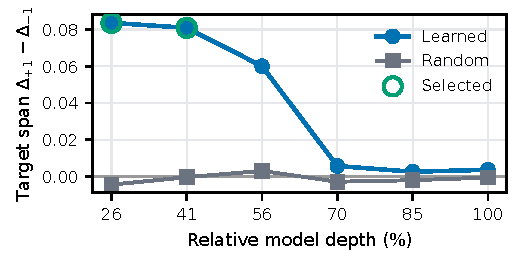
\includegraphics[width=0.96\columnwidth]{figures/layer_selection_profile.pdf}
\caption{Layer selection on a 500-record subset. Target-margin span across relative depth identifies blocks 7 and 11 as the strongest distinct middle-depth blocks; random spans remain near zero.}
\label{fig:layer-selection}
\end{figure}

\begin{table*}[!t]
\centering
\small
\renewcommand{\arraystretch}{0.88}
\setlength{\tabcolsep}{1.4pt}
\caption{Random-calibrated path incidence (\%) for the 3,000-record primary study and three 500-record confirmations. N/C-dmg. are collateral damage; $\Delta$ columns are learned-minus-random points. Bold marks each block's strongest learned result.}
\label{tab:main-results}
\begin{tabular*}{\textwidth}{@{\extracolsep{\fill}}clrrrrrrrrrr@{}}
\toprule
Layer & Direction & Supp. & Enh. & Target & N-dmg. & C-dmg. & Cl. supp. & Cl. enh. & Clean & $\Delta$T & $\Delta$C \\
\midrule
\multicolumn{12}{c}{\textbf{A. Qwen3-1.7B-Base} \quad ($n=3,000$, primary scale, $\tau_T=0.175$)} \\
\cmidrule(lr){1-12}
7 & Random & 5.1 & 4.7 & 9.5 & 8.2 & 8.2 & 4.7 & 4.3 & 8.9 & -- & -- \\
7 & Mean diff. & 6.1 & 7.0 & 12.8 & 7.9 & 8.2 & 5.6 & 6.7 & 12.0 & +3.3 & +3.2 \\
7 & Logistic & 6.7 & 6.1 & 12.4 & 9.1 & 9.0 & 6.3 & 5.7 & 11.6 & +2.8 & +2.8 \\
7 & Linear & 5.8 & 6.2 & 11.6 & 8.8 & 8.4 & 5.2 & 6.0 & 10.8 & +2.1 & +2.0 \\
7 & RFM/AGOP & 7.1 & 6.4 & \textbf{13.1} & 8.5 & 9.0 & 6.5 & 6.1 & \textbf{12.3} & \textbf{+3.6} & \textbf{+3.4} \\
\addlinespace[0.35pt]
11 & Random & 4.7 & 4.2 & 8.8 & 7.0 & 7.1 & 4.5 & 3.8 & 8.3 & -- & -- \\
11 & Mean diff. & 6.2 & 5.3 & \textbf{11.3} & 7.8 & 7.1 & 5.6 & 5.1 & \textbf{10.6} & \textbf{+2.5} & \textbf{+2.3} \\
11 & Logistic & 5.7 & 5.7 & 11.2 & 7.4 & 7.1 & 5.4 & 5.4 & \textbf{10.6} & +2.4 & \textbf{+2.3} \\
11 & Linear & 5.3 & 5.1 & 10.2 & 6.8 & 7.1 & 5.0 & 4.9 & 9.7 & +1.4 & +1.4 \\
11 & RFM/AGOP & 5.1 & 5.3 & 10.2 & 7.5 & 7.2 & 4.8 & 5.1 & 9.7 & +1.4 & +1.5 \\
\midrule
\multicolumn{12}{c}{\textbf{B. Qwen3-1.7B-Base} \quad ($n=500$, residual-norm matched, $\tau_T=0.177$)} \\
\cmidrule(lr){1-12}
7 & Random & 4.4 & 4.8 & 9.0 & 7.4 & 9.2 & 4.0 & 4.0 & 7.8 & -- & -- \\
7 & Mean diff. & 5.2 & 7.4 & 12.6 & 8.2 & 10.2 & 4.4 & 7.2 & 11.6 & +3.6 & +3.8 \\
7 & Logistic & 6.8 & 6.2 & 12.8 & 8.0 & 8.6 & 6.6 & 5.6 & 12.0 & +3.8 & +4.2 \\
7 & RFM/AGOP & 6.2 & 7.8 & \textbf{13.2} & 9.4 & 9.6 & 5.6 & 7.2 & \textbf{12.4} & \textbf{+4.2} & \textbf{+4.6} \\
\addlinespace[0.35pt]
11 & Random & 4.8 & 4.8 & 9.6 & 7.6 & 9.0 & 4.8 & 4.4 & 9.2 & -- & -- \\
11 & Mean diff. & 6.0 & 4.6 & 10.0 & 7.6 & 8.0 & 5.0 & 4.2 & 8.6 & +0.4 & -0.6 \\
11 & Logistic & 5.8 & 6.4 & \textbf{12.2} & 7.8 & 7.4 & 5.6 & 5.8 & \textbf{11.4} & \textbf{+2.6} & \textbf{+2.2} \\
11 & RFM/AGOP & 4.2 & 5.8 & 9.8 & 8.2 & 7.4 & 3.8 & 5.2 & 8.8 & +0.2 & -0.4 \\
\midrule
\multicolumn{12}{c}{\textbf{C. Qwen3.5-2B-Base} \quad ($n=500$, residual-norm matched, $\tau_T=0.111$)} \\
\cmidrule(lr){1-12}
6 & Random & 4.6 & 4.0 & 8.6 & 7.6 & 8.2 & 3.6 & 3.6 & 7.2 & -- & -- \\
6 & Mean diff. & 16.6 & 17.2 & 30.2 & 9.6 & 8.8 & 14.6 & 16.0 & 28.2 & +21.6 & +21.0 \\
6 & Logistic & 18.8 & 16.0 & 28.4 & 11.2 & 5.6 & 17.0 & 15.2 & 26.8 & +19.8 & +19.6 \\
6 & RFM/AGOP & 18.8 & 17.6 & \textbf{32.0} & 10.6 & 9.0 & 17.8 & 17.4 & \textbf{31.2} & \textbf{+23.4} & \textbf{+24.0} \\
\addlinespace[0.35pt]
9 & Random & 4.6 & 4.8 & 9.4 & 6.8 & 5.4 & 4.2 & 4.4 & 8.6 & -- & -- \\
9 & Mean diff. & 9.2 & 7.2 & 15.6 & 9.6 & 5.2 & 8.8 & 6.8 & \textbf{15.0} & +6.2 & \textbf{+6.4} \\
9 & Logistic & 7.8 & 8.8 & \textbf{16.2} & 8.6 & 6.0 & 7.0 & 8.0 & 14.6 & \textbf{+6.8} & +6.0 \\
9 & RFM/AGOP & 8.0 & 7.4 & 15.0 & 9.0 & 5.8 & 7.4 & 6.6 & 13.8 & +5.6 & +5.2 \\
\midrule
\multicolumn{12}{c}{\textbf{D. Ministral-3-3B-Base} \quad ($n=500$, residual-norm matched, $\tau_T=0.083$)} \\
\cmidrule(lr){1-12}
6 & Random & 6.2 & 5.0 & 10.6 & 7.8 & 9.4 & 5.6 & 4.6 & 9.8 & -- & -- \\
6 & Mean diff. & 11.2 & 11.2 & 21.2 & 10.6 & 9.8 & 10.4 & 10.6 & 19.8 & +10.6 & +10.0 \\
6 & Logistic & 10.0 & 12.2 & \textbf{21.4} & 11.2 & 8.8 & 9.8 & 11.6 & \textbf{20.6} & \textbf{+10.8} & \textbf{+10.8} \\
6 & RFM/AGOP & 11.0 & 9.8 & 19.4 & 11.2 & 11.4 & 10.4 & 9.2 & 18.2 & +8.8 & +8.4 \\
\addlinespace[0.35pt]
10 & Random & 3.6 & 4.6 & 7.8 & 7.2 & 8.8 & 3.2 & 4.6 & 7.4 & -- & -- \\
10 & Mean diff. & 9.0 & 8.0 & 16.4 & 8.4 & 6.4 & 8.8 & 7.4 & 15.6 & +8.6 & +8.2 \\
10 & Logistic & 9.6 & 8.6 & \textbf{17.8} & 8.8 & 9.2 & 9.0 & 8.2 & \textbf{16.8} & \textbf{+10.0} & \textbf{+9.4} \\
10 & RFM/AGOP & 8.6 & 8.2 & 16.0 & 7.6 & 8.0 & 8.0 & 7.4 & 14.8 & +8.2 & +7.4 \\
\bottomrule
\end{tabular*}

\end{table*}


\subsection{Learned Directions Improve Selective Paths}

Table~\ref{tab:main-results} reports both the powered 3,000-record outcome
estimate and the three pre-specified 500-record confirmations. Its entries are
path-incidence percentages; $\Delta$T and $\Delta$C are percentage-point
differences from the within-model random control, not AUROC. In the primary
study, layer-7 RFM/AGOP reaches \textbf{13.1\% Target and 12.3\% Clean}, the
strongest selective-path result. More broadly, learned directions improve
target leverage and clean-path incidence over random controls. The strongest
construction varies by block.

Record-paired bootstrap intervals confirm the learned-over-random Target and
Clean gains for the strongest primary-study directions. Collateral incidence
varies by model and layer; full intervals are reported in the Supplementary
Material.

The residual-norm-matched confirmations preserve the same qualitative pattern
at model-dependent magnitudes. Figure~\ref{fig:path-outcome-profiles} shows
that learned directions generally increase target leverage, while collateral
incidence varies across models and layers. The Qwen3-1.7B subset also closely
tracks the powered estimate, separating cohort variation from the cross-model
scale alignment.

\subsection{Low-Dose Responses Forecast Later Outcomes}

Prediction is the central test of PML. Static localization is a weak prior:
Figure~\ref{fig:cross-model-prediction-heatmap} establishes a consistent
diagnostic hierarchy. Static localization $L$ adds little beyond base and metadata
features, while supervised geometry $G$ offers a similarly limited gain. In
contrast, the strength-disjoint weak response $R$ produces the dominant gain
across outcomes and models. The Supplementary Material further separates this
gain from ordinary scalar weak-to-strong correlation. Positive-label prevalence
is 8--11\%, so the reported tables include AP with AUROC. For Target-any and
Clean-any, a multivariate $R$-only random forest substantially improves on a
single signed response, with the complete predictor adding a smaller final
gain. Final macro AUROC remains around \textbf{0.80--0.85} under record-,
dataset-, and domain-held-out evaluation. Removing all 500 records used for
layer selection leaves the four principal full-predictor AUROCs within 0.01 of
the 3,000-record estimates. The same predictive ordering therefore holds after
removing the layer-selection records: a structured low-dose causal response is
more informative about later paths than static localization geometry alone.

\FloatBarrier

\begin{figure*}[!t]
    \centering
    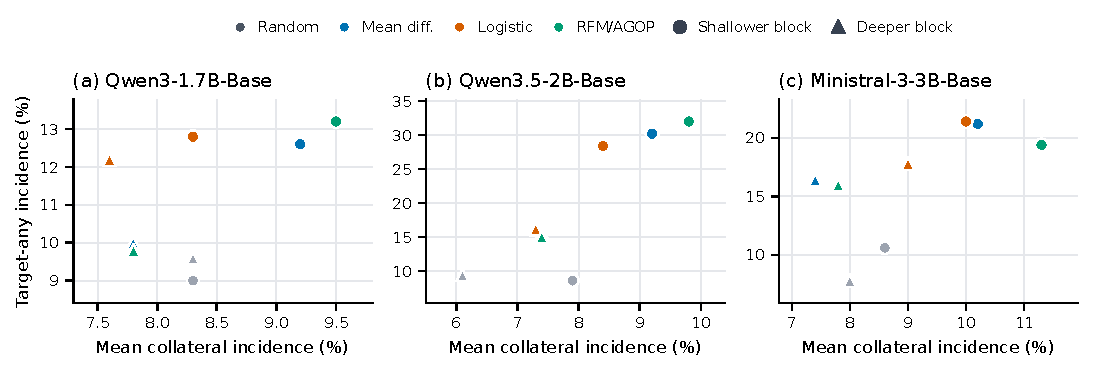
\includegraphics[width=0.89\textwidth]{figures/path_outcome_profiles.pdf}
    \caption{Target leverage and collateral incidence on the common 500-record
    cohort. Each panel shows one base model; colors identify direction
    construction and marker shapes identify the shallower or deeper
    pre-specified block. The vertical axis is Target-any path incidence, while
    the horizontal axis averages semantic-neighbor and capability-damage
    incidence. Each model has two pre-specified block evaluations, with
    panel-specific axes that keep within-model trade-offs visible.}
    \label{fig:path-outcome-profiles}
\end{figure*}

\begin{figure*}[!t]
    \centering
    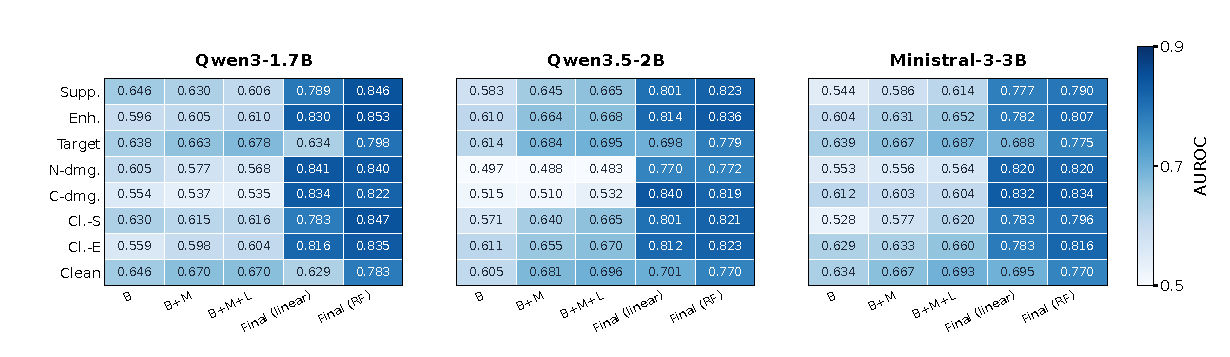
\includegraphics[width=\textwidth]{figures/cross_model_prediction_heatmap.pdf}
    \caption{Cross-model path prediction. Per-outcome record-held-out
    AUROC on the common 500-record cohort. The first three random-forest columns
    cumulatively add base margins and record descriptors ($B$), method/block
    metadata ($M$), and static localization ($L$). The final two columns use the
    complete $B{+}M{+}L{+}R$ features with a linear predictor or random forest,
    providing a predictor-class ablation. The weak response produces the
    dominant feature gain under both predictors, while the nonlinear model gives
    the strongest final performance.}
    \label{fig:cross-model-prediction-heatmap}
\end{figure*}

\subsection{Forecasts Improve Strength Decisions}

We train candidate-strength models from complementary dense and sparse
trajectories, then evaluate on disjoint dense-grid records. Before a candidate
outcome is revealed, each policy selects one coefficient or abstains. The
Supplementary Material gives the full 100-record proof-of-concept table.
Relative to a train-tuned fixed coefficient, utility improves by \textbf{0.055}
and \textbf{0.034}, mainly as neighbor damage falls from 6.0\% to 1.8\% and
5.2\% to 2.2\%. Suppression exceeds no intervention, while enhancement shows
a positive but uncertain gain. The policy averages 2.55/2.61 coefficient evaluations---two
weak probes plus a final action---versus 26 for a dense scan; shared direction
fitting is excluded. Weight sensitivity and full outcomes are supplementary.

\subsection{Endpoint Scope}

Free-generation stress tests are reported in the Supplementary Material. They
show that margin movement can alter text, while wrong-to-right correction is
less frequent. PML therefore evaluates teacher-forced,
margin-level intervention paths.
